\documentclass[a4paper, 12pt]{article}


\usepackage{times}
\usepackage{amssymb}
\usepackage{amsmath}
\usepackage{latexsym}
\usepackage{stmaryrd}
\usepackage{soul}
\usepackage{graphicx}
\graphicspath{ {images/} }


\begin{document} 
\author{Kate Trofimova,  Miro Banovic}
\title{Project Documentation: Web Scraping and Analyzing very large Web server log files}
\date{\today}
\pagenumbering{roman}

\maketitle
\titlepage
\cleardoublepage

\thispagestyle{plain}
\setcounter{page}{2}
\tableofcontents
\cleardoublepage

\listoffigures
\cleardoublepage

\pagenumbering{arabic}

\section{Introduction}
For the course Software Engineering for Economists we received a team assignment entailing the coding, documentation and description of a computer program. Having started out with 4 team members, our team now only consists of Kate Trofimova and Miro Banovic, as two of our colleagues dropped the course. Nonetheless, we set out to write a meaningful program while paying heed to the contents of the course. 

In this, however, the two of us have very different pre-knowledge, which is why for us a significant part of the assignment also encompassed the mutual understanding of different aspects. Therefore, we decided that Miro Banovic would attempt to code the different parts of our final project and write this project documentation and description. As Kate Trofimova is significantly more advanced with regards to programming, she will then correct and improve everything. To facilitate the work process and due to the fact that we are only two team members, this process is very iterative and we often meet to work together. 

Eventually, such process results in a program that scraps and analyzes large data sets from websites. We deem this to be an important task for our personal learning as well as one fitting the requirements of the course, as there are millions of different expert forums on the internet and finding a way to analyze these from the outset could be important. While initially the plan was to write only a MapReduce program utilizing already collected datasets, we later decided to expand the scope of the project and collect the data ourselves by writing a web scraping program. 

In the following, first a description of this thought process and how exactly we came up with the idea will be given, including the general purpose of our program and why it is useful. Then, a more detailed explanation of the programs chracteristics will be given, followed by a depiction of what libraries were used and how the process can be replicated by Prof. Dr. Zahn.
\cleardoublepage

\section{Thought Process}
In this section, we will describe how we came up with the idea to write a web scraper as well as a MapReduce program using Hadoop. Due to the aforementioned diverging levels of knowledge, one important factor for us was that we will both be able to contribute to the project. However, because especially Kate Trofimova is highly ambitious with regards to this course, at the same time we also wanted to have a challenging as well as rewarding tasks. In this, we thought about personal interests and needs, eventually leading to our decision to move forward with a data analysis program. This idea is inspired by the Udacity course "Intro to Hadoop and MapReduce", which we also used to gain knowledge with regard to the topic and its importance.

We deem our program to be of use not only to ourselves but also in general, as there are incredible amounts of data available on the internet. These, however, are not always easy to extract from the corresponding websites and doing so manually is an extremely time-intensive job. Further, with the emergence of big data in recent years, analysis of large data sets takes increasingly much time as well as computing power. And although according to Moore's Law computing power becomes cheaper and cheaper (Moore, 1965), this exponential increase in data leads to the necessity to use several machines at the same time to analyze such data. 

Taken together, our program will allow us and other users to obtain information from a website and then analyze this information using several computers or servers. Through this the information underlying such data becomes more accessible, and with only a few tweaks the program can be adapted to other websites.

While the web scraper will be a stand-alone program which can be run on a single machine, MapReduce consist of both a mapper and a reducer. Thus, overall we will be programming:
\begin{enumerate}
	\item Web scraper
	\item Mapper
	\item Reducer
\end{enumerate}
All of this is done using python, and we decided to communicate through slack and use github to share files. Having made our thought process and ideation of the project clear, in the following section the aspects of the three different programs as described above will be detailed.
\cleardoublepage

\section{Programs}
Creating three different but interrelated programs increases the workload, but at the same time facilitates the division of tasks and enables us to learn. As these programs will have to be run and replicated by Prof. Dr. Zahn, in the following we will first describe how these are connected and then go into more detailed descriptions of the individual parts. 

\subsection{Connection}
Inititally, we wanted to only write a MapReduce program and saw this as challenging enough, especially because the two members of our team who later dropped the course were even less advanced than Miro Banovic with regards to coding. Once these members had left the team and the rest of us started looking into and learning more about Hadoop and MapReduce with help of the aforementioned Udacity course, we quickly understood that although such program is definitely challenging as well as useful, the scope of such a tasks did not suffice in our eyes. Mapper and Reducer, while computationally demanding and being used in real companies, each consist of only relatively few lines of code. Furthermore, using these two programs alone requires the existence of a dataset. This would make the tasks quite generic if we were to choose a random dataset, which is why it made perfect sense to us to take a step back and collect such data ourselves. 

Taken together, these three programs now allow for the collection as well as analysis of (large) datasets from any given website, with a few adaptations. Our program specifically was written to obtain information from the website WEBSITEDOMAIN, which is why we strongly urge users to replicate our process on the same website before adapting the program for other information sources.

\subsection{Web scraper}
Per se, web pages are built to be used by human end-users and not by automated software. Due to this, much of the data these websites contain is in the form of text easily understandable for humans, while the sites themselves are built using mark-up languages such as HTML. To analyze such data, however, it needs to be extracted from the web page and put into structured form. 

In its most basic form, web scraping is copy-paste actions performed manually by a human user. While this approach is oftentimes appropriate when human judgment is needed, it is extremely time consuming especially for bigger datasets. To automate this process, a program that is both fetching the website and extracting the data from it is needed (Boeing and Waddell, 2016). 

Through this, the data will be put in some sort of structured format and thus can be analyzed more easily by automated programs. Exactly this is what our initial idea of a MapReduce program was about, which is why we deemed a web scraper to be an appropriate first step to expand the scope of the assignment. The next steps in analyzing these big data sets are a mapper and a reducer which together make up the MapReduce system and are described in the following.

\subsection{MapReduce}
Mapper and reducer are generally used together in order to allow for several machines to analyze a big data set. As such, the initial data set is split up and the created sub-sets are analyzed individually by different machines, before the information gathered from the sub-sets is again out together in a last step. The following figure visualizes this procedure, in which the first step is handled by the Mapper and the second step is done by the reducer. 

\begin{figure}[h]
\centering
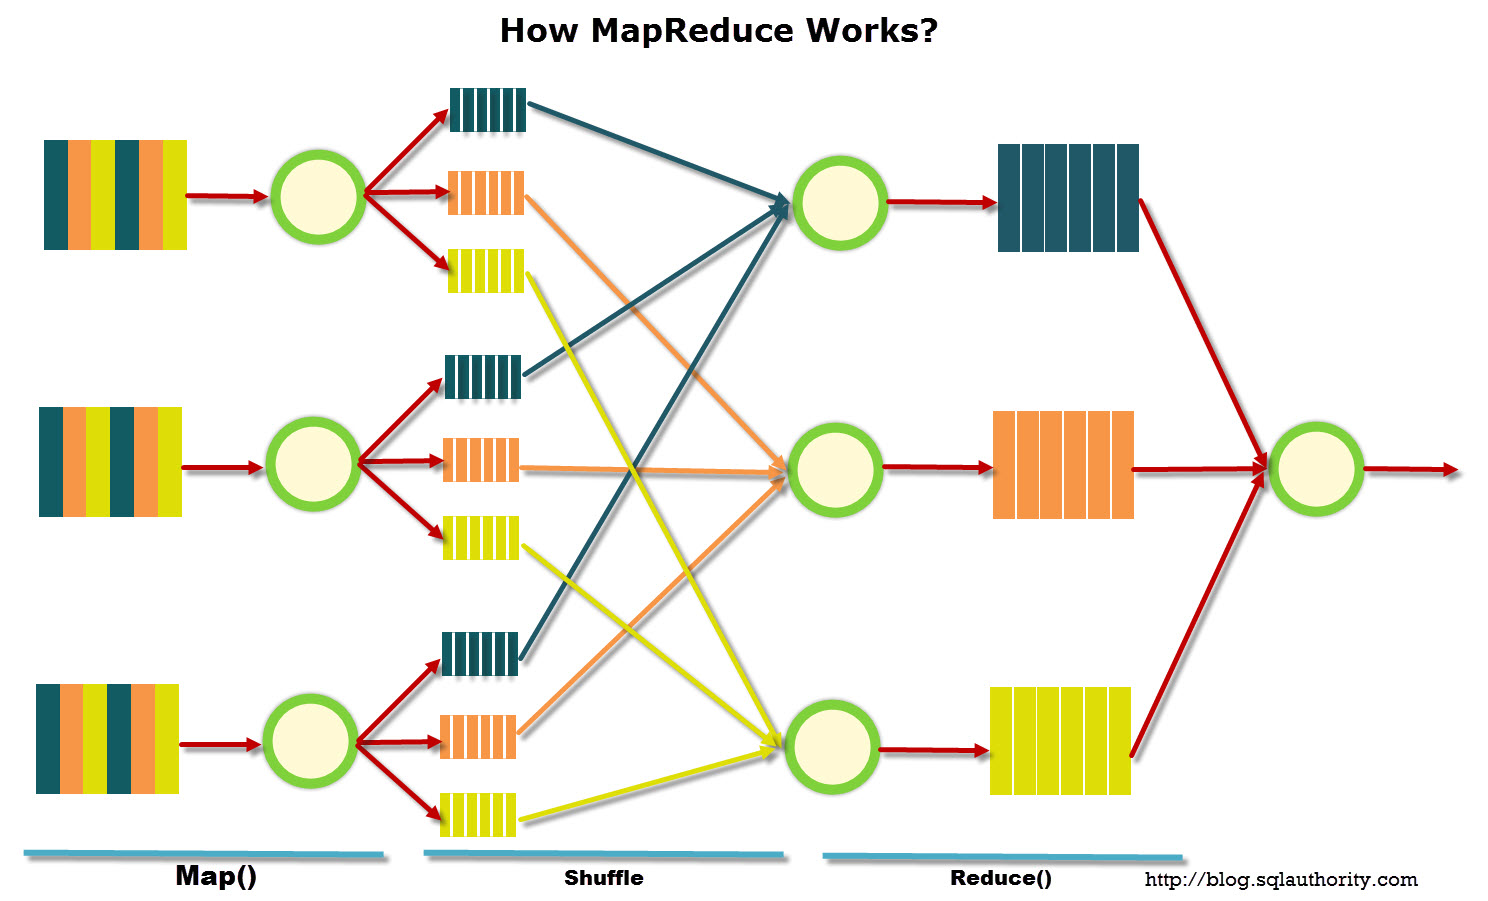
\includegraphics[width=1\textwidth]{mapreduce}
\caption{Visualization of MapReduce (Blog.sqlauthority.com, 2013)}
\end{figure}

\subsubsection{Mapper}
"Mapper maps input key/value pairs to a set of intermediate key/value pairs. [...] Output pairs do not need to be of the same types as input pairs. A given input pair may map to zero or many output pairs. [...] All intermediate values associated with a given output key are subsequently grouped by the framework, and passed to the Reducer(s) to determine the final output" (Hadoop.apache.org, 2013). 

\subsubsection{Reducer}
"Reducer reduces a set of intermediate values which share a key to a smaller set of values. [...] Reducer has 3 primary phases: shuffle, sort and reduce. 
\begin{itemize}
	\item Shuffle

Input to the Reducer is the sorted output of the mappers. In this phase the framework fetches the relevant partition of the output of all the mappers, via HTTP.
	\item Sort

The framework groups Reducer inputs by keys (since different mappers may have output the same key) in this stage. The shuffle and sort phases occur simultaneously; while map-outputs are being fetched they are merged.
	\item Reduce

In this phase the reduce(WritableComparable, Iterator, OutputCollector, Reporter) method is called for each <key, (list of values)> pair in the grouped inputs. The output of the Reducer is not sorted." (Hadoop.apache.org, 2013)
\end{itemize}

\section{How to use?}
A few general sentences about this section

\subsection{Libraries used}
Description about what libraries were used and why/how

\subsection{Other subsections}

\cleardoublepage
\pagenumbering{alph}
\addcontentsline{toc}{section}{References}
\begin{thebibliography}{1}
\bibitem{latexcompanion} 
Moore, G. E. (1965). Cramming More Components Onto Integrated Circuits. \textit{Electronics,} 38(8).
\bibitem{latexcompanion} 
Boeing, G.; Waddell, P. (2016). New Insights into Rental Housing Markets across the United States: Web Scraping and Analyzing Craigslist Rental Listings. Journal of Planning Education and Research. \textit{Journal of Planning Education and Research.}
\bibitem{latexcompanion}
Hadoop.apache.org. (2013). [online] Available at: https://hadoop.apache.org/ [Accessed 22 Dec. 2017]. 
\bibitem{latexcompanion}
Blog.sqlauthority.com. (2017). \textit{Big Data - Buzz Words: What is MapReduce.} [online] Available at: https://blog.sqlauthority.com/2013/10/09/big-data-buzz-words-what-is-mapreduce-day-7-of-21/ [Accessed 22 Dec. 2017].

\end{thebibliography}

\end{document}